% Influence of different pedestrian flux densities

\noi For this experiment we monitored the total agents count as an indicator for jams. This number was then scaled by the combined flux densities to give comparable results which can be found in figure \ref{fig:AAllAveragesScaled}. An unscaled version of this is figure \ref{fig:AAllAveragesInOnePlot}, where one can see the same effects as well as the average number in the system being almost parallel to each other.\\
\begin{figure}[h!]
	\centering
		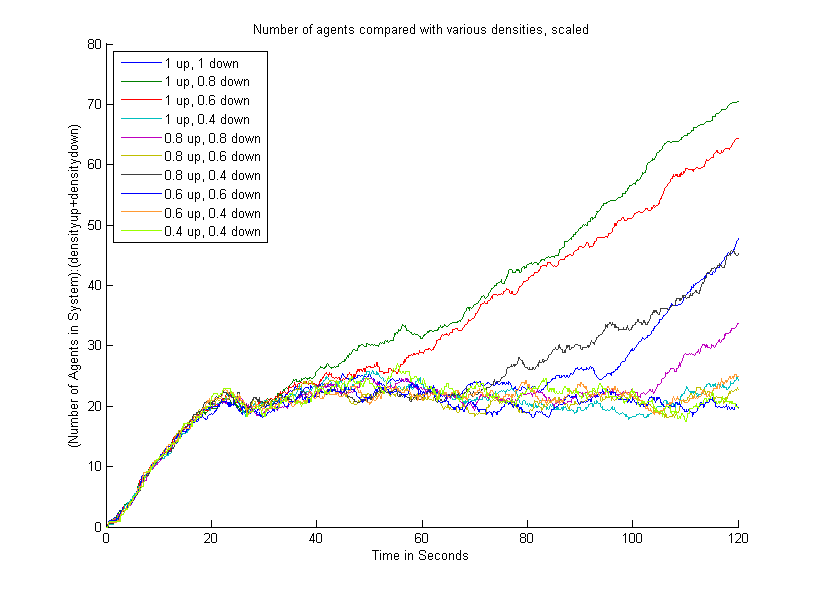
\includegraphics[width=0.80\textwidth]{pictures/AAllAveragesScaled.png}
	\caption{The scaled total number of agents in the system for various combinations of flux densities with respect to time. The used flux densities are given in the graph legend. As soon as the total number of agents runs away, a jam has formed. The mean over three simulations with different seeds was taken for each case. As expected, high flux densities caused massive jams.}
	\label{fig:AAllAveragesScaled}
\end{figure}

\noi With the highest flux densities used in the simulations, the jam formation was very fast. It is interesting that 0.6/0.6, 0.8/0.4 and 0.8/0.8 also caused jams within the observed time frame, especially since 1/0.4 didn't jam.\\
Our model seems not to be able to cope well with that many people. There should be more simulations with different seeds to get a better statistic.\\

\begin{figure}[h!]
	\centering
		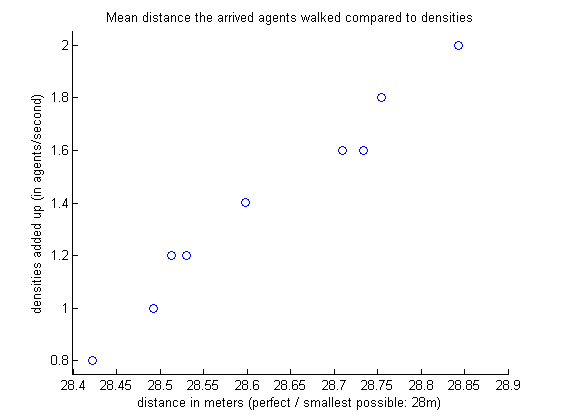
\includegraphics[width=0.49\textwidth]{pictures/AMeanDistancesCompared.png}
		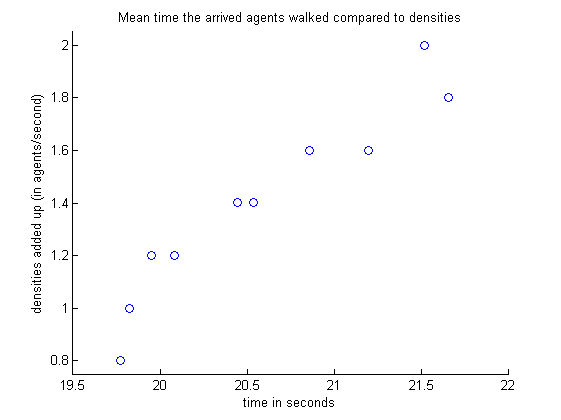
\includegraphics[width=0.49\textwidth]{pictures/AMeanTimeCompared.png}
	\caption{Graphs of the mean covered distance and mean time spent during the simulation for all agents who reached their destruction line compared with the combined flux densities used. As expected, for high flux densities the agents have to cover longer distances and spend more time as they have to avoid colliding with other agents. Note that even though this data is interestingly distributed, its statistical relevance is rather small, because the standard deviation is rather high due to the agent's speeds being Gaussian distributed.}
	\label{fig:ACompared}
\end{figure}

\noi Given in figure \ref{fig:ACompared} are the mean covered distance and mean time spent during the simulation for all agents who reached their destruction line compared with the combined flux densities used. As would be expected, the agents had to cover a longer distance and spend more time in the simulation as they had to avoid collisions with other agents.\\
These variables were monitored to analyze whether they give a good description of the model and to ensure that we got results that run within the same expectations as in reality. But as they only take the values of those agents that have left the simulation, they may have a decreased significance when jams occur and are not at all able to tell whether a jam has occured or not.\\

\noi To sum up, we could observe what we expected to see: the more people, the more probably a jam pops up. Also, when the densities are increased, the agents have to walk longer ways, need a bit more time and thus have a smaller average velocity.
